\documentclass{standalone}
\usepackage{tikz}
\usetikzlibrary{patterns, positioning}
\usepackage[sfdefault]{ClearSans} %% option 'sfdefault' activates Clear Sans as the default text font
\usepackage[T1]{fontenc}

\begin{document}
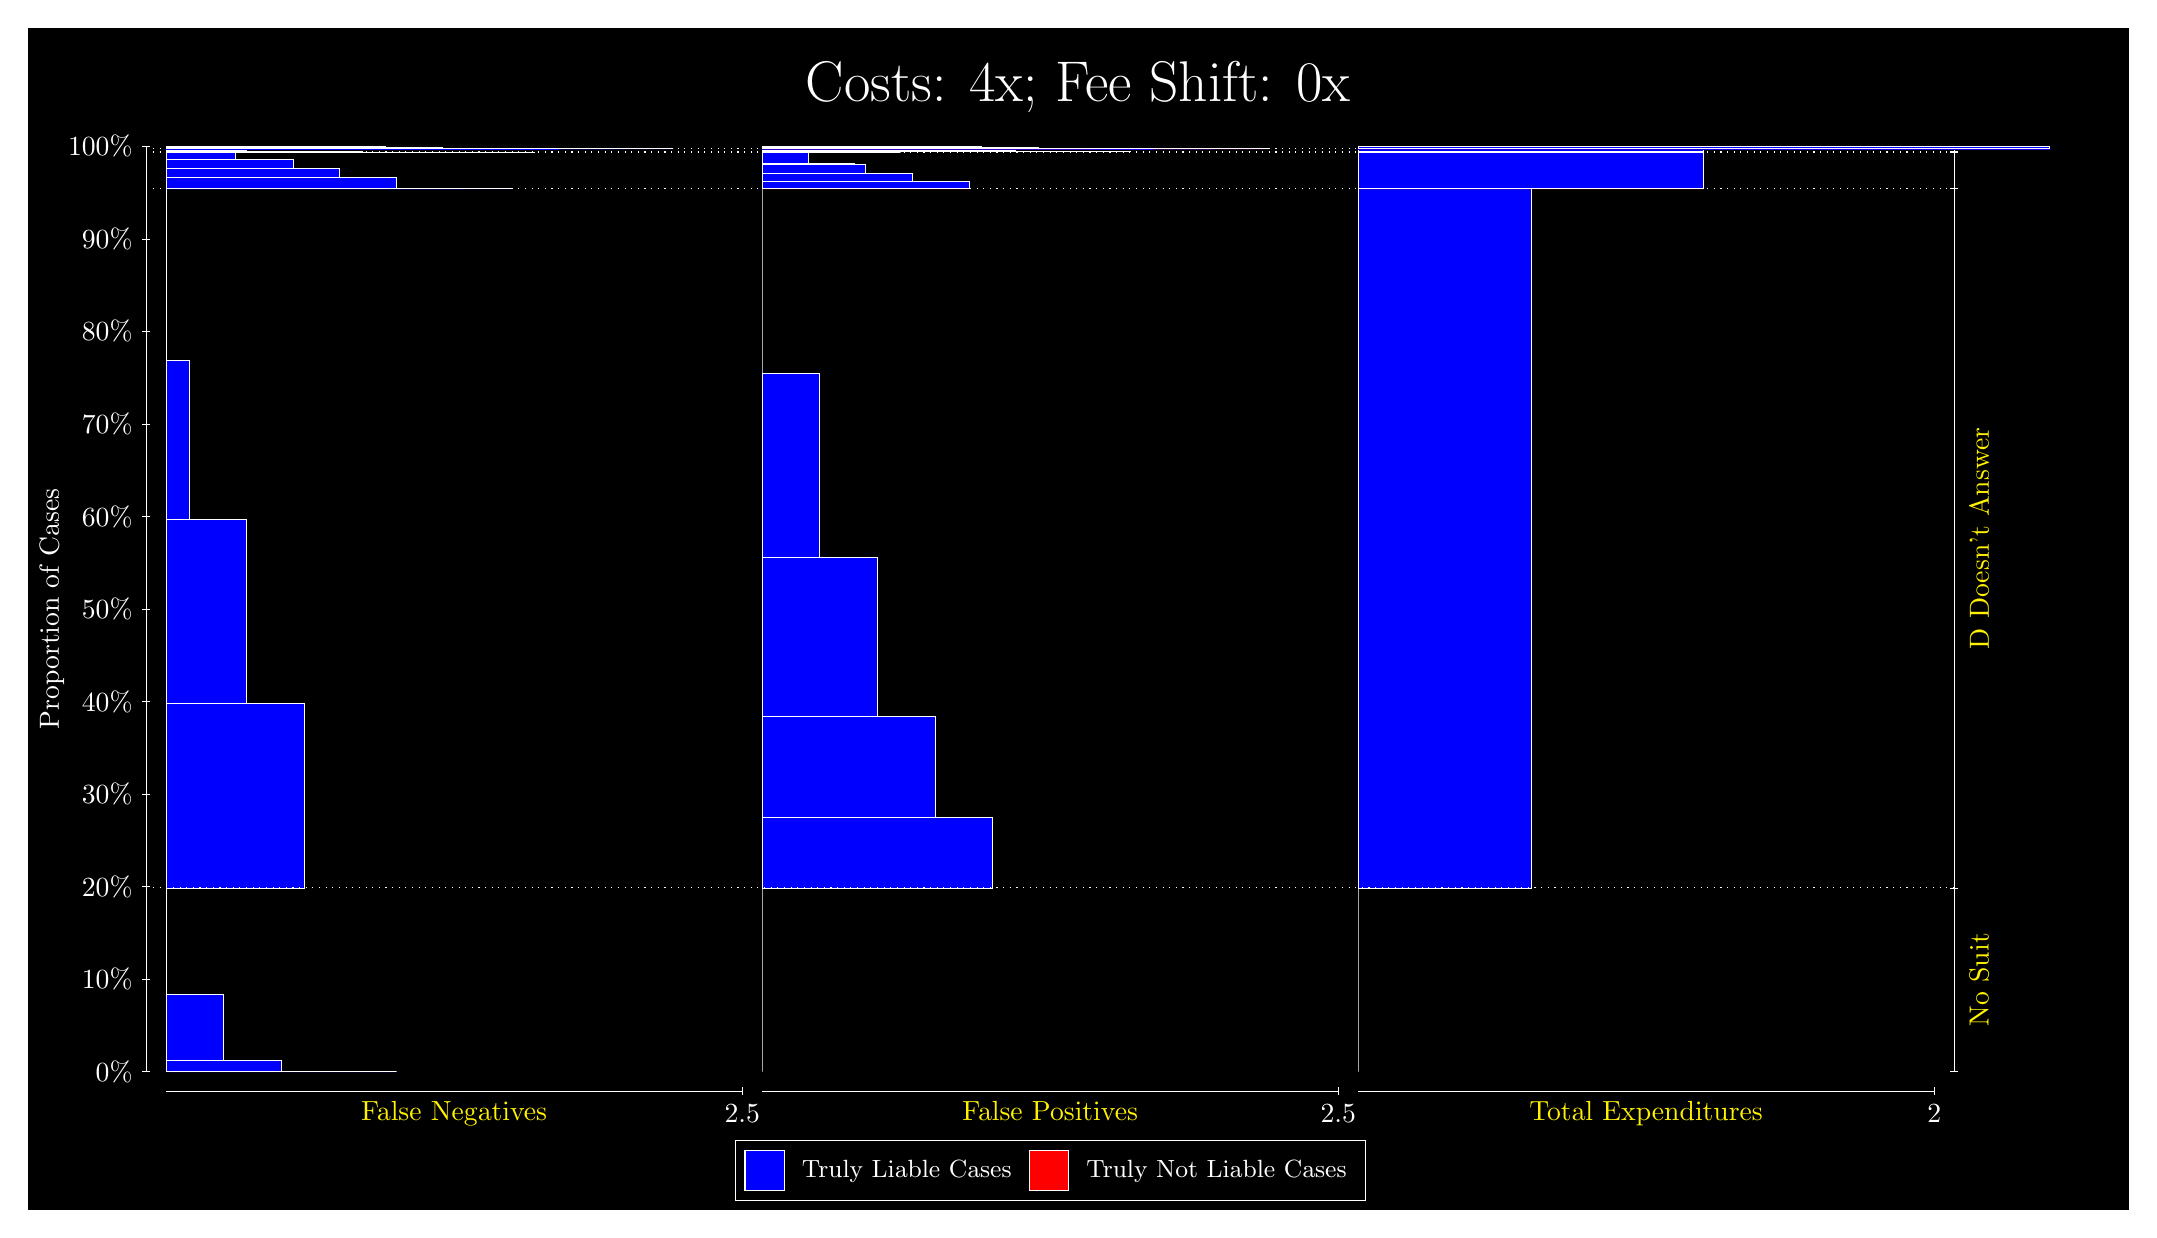
\begin{tikzpicture}
\draw[fill=black] (0,0) rectangle (26.667,15);
\draw[text=white] (0,13.5) rectangle (26.667,15) node[midway] {\huge Costs: 4x; Fee Shift: 0x};
\draw[white, very thin] (1.5,1.75) -- (1.5,13.5);
\node[rotate=90, text=white, anchor=center] at (0.3, 7.625) {Proportion of Cases};
\draw[white, very thin] (1.45,1.75) -- (1.55,1.75);
\node[text=white, anchor=east] at (1.45, 1.75) {0\%};
\draw[white, very thin] (1.45,2.925) -- (1.55,2.925);
\node[text=white, anchor=east] at (1.45, 2.925) {10\%};
\draw[white, very thin] (1.45,4.1) -- (1.55,4.1);
\node[text=white, anchor=east] at (1.45, 4.1) {20\%};
\draw[white, very thin] (1.45,5.275) -- (1.55,5.275);
\node[text=white, anchor=east] at (1.45, 5.275) {30\%};
\draw[white, very thin] (1.45,6.45) -- (1.55,6.45);
\node[text=white, anchor=east] at (1.45, 6.45) {40\%};
\draw[white, very thin] (1.45,7.625) -- (1.55,7.625);
\node[text=white, anchor=east] at (1.45, 7.625) {50\%};
\draw[white, very thin] (1.45,8.8) -- (1.55,8.8);
\node[text=white, anchor=east] at (1.45, 8.8) {60\%};
\draw[white, very thin] (1.45,9.975) -- (1.55,9.975);
\node[text=white, anchor=east] at (1.45, 9.975) {70\%};
\draw[white, very thin] (1.45,11.15) -- (1.55,11.15);
\node[text=white, anchor=east] at (1.45, 11.15) {80\%};
\draw[white, very thin] (1.45,12.325) -- (1.55,12.325);
\node[text=white, anchor=east] at (1.45, 12.325) {90\%};
\draw[white, very thin] (1.45,13.5) -- (1.55,13.5);
\node[text=white, anchor=east] at (1.45, 13.5) {100\%};

\draw[white, very thin] (24.457,1.75) -- (24.457,13.5);
\draw[white, very thin] (24.407,1.75) -- (24.507,1.75);
\node[anchor=west] at (24.407, 1.75) {};
\draw[white, very thin] (24.407,4.0822) -- (24.507,4.0822);
\node[anchor=west] at (24.407, 4.0822) {};
\draw[white, very thin] (24.407,12.963) -- (24.507,12.963);
\node[anchor=west] at (24.407, 12.963) {};
\draw[white, very thin] (24.407,13.425) -- (24.507,13.425);
\node[anchor=west] at (24.407, 13.425) {};
\draw[white, very thin] (24.407,13.436) -- (24.507,13.436);
\node[anchor=west] at (24.407, 13.436) {};
\draw[white, very thin] (24.407,13.469) -- (24.507,13.469);
\node[anchor=west] at (24.407, 13.469) {};
\draw[white, very thin] (24.407,13.5) -- (24.507,13.5);
\node[anchor=west] at (24.407, 13.5) {};

\draw[white, very thin, fill=blue] (1.75,1.75) rectangle (4.6775,1.75);
\draw[white, very thin, fill=blue] (1.75,1.75) rectangle (3.9457,1.7512);
\draw[white, very thin, fill=blue] (1.75,1.7512) rectangle (3.2138,1.8918);
\draw[white, very thin, fill=blue] (1.75,1.8918) rectangle (2.4819,2.7256);
\draw[white, very thin, fill=red] (1.75,2.7256) rectangle (1.75,2.7256);
\draw[white, very thin, fill=blue] (1.75,2.7256) rectangle (1.75,4.0822);
\draw[white, very thin, fill=blue] (1.75,4.0822) rectangle (3.5065,6.4319);
\draw[white, very thin, fill=blue] (1.75,6.4319) rectangle (2.7746,8.7632);
\draw[white, very thin, fill=blue] (1.75,8.7632) rectangle (2.0428,10.784);
\draw[white, very thin, fill=red] (1.75,10.784) rectangle (1.75,10.784);
\draw[white, very thin, fill=blue] (1.75,10.784) rectangle (1.75,12.963);
\draw[white, very thin, fill=blue] (1.75,12.963) rectangle (6.1413,12.963);
\draw[white, very thin, fill=blue] (1.75,12.963) rectangle (5.5558,12.963);
\draw[white, very thin, fill=blue] (1.75,12.963) rectangle (5.4094,12.966);
\draw[white, very thin, fill=blue] (1.75,12.966) rectangle (4.8239,12.966);
\draw[white, very thin, fill=blue] (1.75,12.966) rectangle (4.6775,13.103);
\draw[white, very thin, fill=blue] (1.75,13.103) rectangle (4.092,13.11);
\draw[white, very thin, fill=blue] (1.75,13.11) rectangle (3.9457,13.224);
\draw[white, very thin, fill=blue] (1.75,13.224) rectangle (3.3602,13.332);
\draw[white, very thin, fill=blue] (1.75,13.332) rectangle (3.2138,13.333);
\draw[white, very thin, fill=blue] (1.75,13.333) rectangle (2.6283,13.425);
\draw[white, very thin, fill=red] (1.75,13.425) rectangle (1.75,13.425);
\draw[white, very thin, fill=blue] (1.75,13.425) rectangle (6.4341,13.425);
\draw[white, very thin, fill=blue] (1.75,13.425) rectangle (5.7022,13.425);
\draw[white, very thin, fill=blue] (1.75,13.425) rectangle (4.9703,13.43);
\draw[white, very thin, fill=blue] (1.75,13.43) rectangle (4.2384,13.436);
\draw[white, very thin, fill=blue] (1.75,13.436) rectangle (3.5065,13.436);
\draw[white, very thin, fill=red] (1.75,13.436) rectangle (1.75,13.436);
\draw[white, very thin, fill=blue] (1.75,13.436) rectangle (3.5065,13.436);
\draw[white, very thin, fill=blue] (1.75,13.436) rectangle (2.7746,13.45);
\draw[white, very thin, fill=blue] (1.75,13.45) rectangle (2.0428,13.467);
\draw[white, very thin, fill=red] (1.75,13.467) rectangle (1.75,13.467);
\draw[white, very thin, fill=blue] (1.75,13.467) rectangle (1.75,13.469);
\draw[white, very thin, fill=blue] (1.75,13.469) rectangle (8.1906,13.469);
\draw[white, very thin, fill=blue] (1.75,13.469) rectangle (7.4587,13.469);
\draw[white, very thin, fill=blue] (1.75,13.469) rectangle (6.7268,13.47);
\draw[white, very thin, fill=blue] (1.75,13.47) rectangle (5.9949,13.477);
\draw[white, very thin, fill=blue] (1.75,13.477) rectangle (5.2631,13.492);
\draw[white, very thin, fill=blue] (1.75,13.492) rectangle (4.5312,13.499);
\draw[white, very thin, fill=blue] (1.75,13.499) rectangle (3.7993,13.5);
\draw[white, very thin, fill=blue] (1.75,13.5) rectangle (3.0674,13.5);
\draw[white, very thin, fill=blue] (1.75,13.5) rectangle (2.3355,13.5);
\draw[white, very thin, fill=red] (1.75,13.5) rectangle (1.75,13.5);
\draw[white, very thin, fill=red] (9.3189,1.75) rectangle (9.3189,1.75);
\draw[white, very thin, fill=blue] (9.3189,1.75) rectangle (9.3189,4.0822);
\draw[white, very thin, fill=red] (9.3189,4.0822) rectangle (12.246,4.0822);
\draw[white, very thin, fill=blue] (9.3189,4.0822) rectangle (12.246,4.9819);
\draw[white, very thin, fill=blue] (9.3189,4.9819) rectangle (11.515,6.2611);
\draw[white, very thin, fill=blue] (9.3189,6.2611) rectangle (10.783,8.282);
\draw[white, very thin, fill=blue] (9.3189,8.282) rectangle (10.051,10.613);
\draw[white, very thin, fill=blue] (9.3189,10.613) rectangle (9.3189,12.963);
\draw[white, very thin, fill=red] (9.3189,12.963) rectangle (11.954,12.963);
\draw[white, very thin, fill=blue] (9.3189,12.963) rectangle (11.954,13.055);
\draw[white, very thin, fill=red] (9.3189,13.055) rectangle (11.368,13.055);
\draw[white, very thin, fill=blue] (9.3189,13.055) rectangle (11.368,13.056);
\draw[white, very thin, fill=blue] (9.3189,13.056) rectangle (11.222,13.164);
\draw[white, very thin, fill=blue] (9.3189,13.164) rectangle (10.636,13.278);
\draw[white, very thin, fill=blue] (9.3189,13.278) rectangle (10.49,13.285);
\draw[white, very thin, fill=blue] (9.3189,13.285) rectangle (9.9044,13.422);
\draw[white, very thin, fill=blue] (9.3189,13.422) rectangle (9.758,13.422);
\draw[white, very thin, fill=blue] (9.3189,13.422) rectangle (9.3189,13.425);
\draw[white, very thin, fill=red] (9.3189,13.425) rectangle (11.075,13.425);
\draw[white, very thin, fill=blue] (9.3189,13.425) rectangle (11.075,13.425);
\draw[white, very thin, fill=blue] (9.3189,13.425) rectangle (10.344,13.43);
\draw[white, very thin, fill=blue] (9.3189,13.43) rectangle (9.6116,13.436);
\draw[white, very thin, fill=blue] (9.3189,13.436) rectangle (9.3189,13.436);
\draw[white, very thin, fill=red] (9.3189,13.436) rectangle (14.003,13.436);
\draw[white, very thin, fill=blue] (9.3189,13.436) rectangle (14.003,13.436);
\draw[white, very thin, fill=blue] (9.3189,13.436) rectangle (13.271,13.439);
\draw[white, very thin, fill=blue] (9.3189,13.439) rectangle (12.539,13.455);
\draw[white, very thin, fill=blue] (9.3189,13.455) rectangle (11.807,13.469);
\draw[white, very thin, fill=blue] (9.3189,13.469) rectangle (11.075,13.469);
\draw[white, very thin, fill=red] (9.3189,13.469) rectangle (15.759,13.469);
\draw[white, very thin, fill=blue] (9.3189,13.469) rectangle (15.759,13.469);
\draw[white, very thin, fill=blue] (9.3189,13.469) rectangle (15.028,13.469);
\draw[white, very thin, fill=red] (9.3189,13.469) rectangle (15.028,13.469);
\draw[white, very thin, fill=blue] (9.3189,13.469) rectangle (15.028,13.469);
\draw[white, very thin, fill=blue] (9.3189,13.469) rectangle (14.296,13.47);
\draw[white, very thin, fill=red] (9.3189,13.47) rectangle (14.296,13.47);
\draw[white, very thin, fill=blue] (9.3189,13.47) rectangle (14.296,13.47);
\draw[white, very thin, fill=blue] (9.3189,13.47) rectangle (13.564,13.47);
\draw[white, very thin, fill=red] (9.3189,13.47) rectangle (13.564,13.47);
\draw[white, very thin, fill=blue] (9.3189,13.47) rectangle (13.564,13.477);
\draw[white, very thin, fill=blue] (9.3189,13.477) rectangle (12.832,13.477);
\draw[white, very thin, fill=red] (9.3189,13.477) rectangle (12.832,13.477);
\draw[white, very thin, fill=blue] (9.3189,13.477) rectangle (12.832,13.492);
\draw[white, very thin, fill=blue] (9.3189,13.492) rectangle (12.1,13.499);
\draw[white, very thin, fill=blue] (9.3189,13.499) rectangle (11.368,13.5);
\draw[white, very thin, fill=blue] (9.3189,13.5) rectangle (10.636,13.5);
\draw[white, very thin, fill=blue] (9.3189,13.5) rectangle (9.9044,13.5);
\draw[white, very thin, fill=red] (16.888,1.75) rectangle (16.888,1.75);
\draw[white, very thin, fill=blue] (16.888,1.75) rectangle (16.888,4.0822);
\draw[white, very thin, fill=red] (16.888,4.0822) rectangle (19.083,4.0822);
\draw[white, very thin, fill=blue] (16.888,4.0822) rectangle (19.083,12.963);
\draw[white, very thin, fill=red] (16.888,12.963) rectangle (21.279,12.963);
\draw[white, very thin, fill=blue] (16.888,12.963) rectangle (21.279,13.425);
\draw[white, very thin, fill=red] (16.888,13.425) rectangle (21.279,13.425);
\draw[white, very thin, fill=blue] (16.888,13.425) rectangle (21.279,13.436);
\draw[white, very thin, fill=red] (16.888,13.436) rectangle (21.279,13.436);
\draw[white, very thin, fill=blue] (16.888,13.436) rectangle (21.279,13.469);
\draw[white, very thin, fill=red] (16.888,13.469) rectangle (25.67,13.469);
\draw[white, very thin, fill=blue] (16.888,13.469) rectangle (25.67,13.47);
\draw[white, very thin, fill=red] (16.888,13.47) rectangle (25.67,13.47);
\draw[white, very thin, fill=blue] (16.888,13.47) rectangle (25.67,13.5);
\draw[white, dotted] (1.5,4.0822) -- (24.457,4.0822);
\draw[white, dotted] (1.5,12.963) -- (24.457,12.963);
\draw[white, dotted] (1.5,13.425) -- (24.457,13.425);
\draw[white, dotted] (1.5,13.436) -- (24.457,13.436);
\draw[white, dotted] (1.5,13.469) -- (24.457,13.469);
\draw[white, very thin] (1.75,1.5) -- (9.0689,1.5);
\node[text=yellow, anchor=north] at (5.4094, 1.5) {False Negatives};
\draw[white, very thin] (9.0689,1.45) -- (9.0689,1.55);
\node[text=white, anchor=north] at (9.0689, 1.45) {2.5};

\draw[white, very thin] (9.3189,1.5) -- (16.638,1.5);
\node[text=yellow, anchor=north] at (12.978, 1.5) {False Positives};
\draw[white, very thin] (16.638,1.45) -- (16.638,1.55);
\node[text=white, anchor=north] at (16.638, 1.45) {2.5};

\draw[white, very thin] (16.888,1.5) -- (24.207,1.5);
\node[text=yellow, anchor=north] at (20.547, 1.5) {Total Expenditures};
\draw[white, very thin] (24.207,1.45) -- (24.207,1.55);
\node[text=white, anchor=north] at (24.207, 1.45) {2};

\node[text=yellow, centered, rotate=90] at (24.777, 2.9161) {No Suit};
\node[text=yellow, centered, rotate=90] at (24.777, 8.5226) {D Doesn't Answer};





\draw (12.978300999999998,1.5) node[draw=none] (baseCoordinate) {};
\begin{scope}[align=center]
        \matrix[scale=0.5, draw=white, below=0.5cm of baseCoordinate, nodes={draw}, column sep=0.1cm]{
            \node[rectangle, draw, minimum width=0.5cm, minimum height=0.5cm, fill=blue] {}; &
            \node[draw=none, font=\small, text=white] (B) {Truly Liable Cases}; &
            \node[rectangle, draw, minimum width=0.5cm, minimum height=0.5cm, fill=red] {}; &
            \node[draw=none, font=\small, text=white] (B) {Truly Not Liable Cases}; \\
            };
\end{scope}

\end{tikzpicture}
\end{document}